% gc-14-IntMeth.tex

\documentclass[xcolor=dvipsnames]{beamer}
\usepackage{teachbeamer}

\title{Integration Methods}
\subtitle{{\CourseNumber}, BCIT}

\author{\CourseName}

\date{April 9, 2018}

\begin{document}

\begin{frame}
  \titlepage
\end{frame}

\begin{frame}
  \frametitle{Integration Methods}
  We will learn about the following integration methods:
  \begin{enumerate}
  \item Using Integration Tables
  \item Integration by Substitution
  \item Integration by Parts
  \item Trigonometric Integrals
  \item Trigonometric Substitutions
  \item Partial Fractions
  \item Improper Integrals
  \end{enumerate}
\end{frame}

\begin{frame}
  \frametitle{Integration by Substitution}
We know how to integrate the following functions
\begin{equation}
  \label{eq:deixugha}
  f_{1}(y)=y^{3}\mbox{ and }f_{2}(x)=2x+5
\end{equation}
but how do you integrate $f=f_{1}\circ{}f_{2}$, for example
\begin{equation}
  \label{eq:eetusiil}
  f(x)=(2x+5)^{3}
\end{equation}
We use the method of \alert{substitution}. Write 
\begin{equation}
  \label{eq:ohshaoxe}
  u=2x+5
\end{equation}
\end{frame}

\begin{frame}
  \frametitle{Integration by Substitution}
Remember that the definition of differentials is as follows. If
$u=f(x)$ and $dx$ is some real number (usually small), then 
\begin{equation}
  \label{eq:eevieweo}
  du=f'(x)\,dx
\end{equation}
The substitution changes \alert{the differential and the limits}. For
$u=2x+5$
\begin{equation}
  \label{eq:ushooxiu}
  du=2dx\mbox{ and therefore }dx=\frac{1}{2}du
\end{equation}
Consequently,
\begin{equation}
  \label{eq:olaihaxi}
  \int_{a}^{b}(2x+5)^{3}\,dx=\int_{2a+5}^{2b+5}u^{3}\cdot{}\frac{1}{2}\,du
\end{equation}
\end{frame}

\begin{frame}
  \frametitle{Integration by Substitution Four Steps}
  \begin{description}
  \item[Step 1: Find Substitution] replace $2x+5$ by $u$ (not all
    expressions involving $x$ have to disappear yet)
  \item[Step 2: Find Substitution for Differential]
    $du=2\cdot{}dx$, therefore $dx=\frac{1}{2}du$
  \item[Step 3: Perform Integration] find $\frac{1}{2}\int{}u^{3}\,du$
  \item[Step 4: Reverse the Substitution] replace $u$ by $2x+5$ in
    the final result for the indefinite integral
  \end{description}
\end{frame}

\begin{frame}
  \frametitle{Integration by Substitution Example}
  \beispiel{Integration by Substitution} Let's evaluate
  \begin{equation}
    \label{eq:eenoophu}
   \int_{0}^{4}x\sqrt{9+x^{2}}\,dx 
  \end{equation}
  We will do this two ways. 
  \begin{description}
  \item[method 1] Find the indefinite integral of $x\sqrt{9+x^{2}}$
    and then use the limits $a=0,b=4$ to evaluate the definite
    integral.
  \item[method 2] Proceed as on the previous slide and change both
    differential \alert{and} limits for the definite interval.
  \end{description}
\end{frame}

\begin{frame}
  \frametitle{Integration by Substitution Example}
  Here is method 1. Substitute $u=9+x^{2}$. Then, $du=2x\,dx$, so
\begin{equation}
  \label{eq:iachuejo}
  \frac{1}{2}\,du=x\,dx
\end{equation}
Notice that we need the factor $x$ on the right-hand side in order to
make this integration work.
\begin{equation}
  \label{eq:diacheiv}
  \int{}x\sqrt{9+x^{2}}\,dx=\frac{1}{2}\int{}\sqrt{u}\,du=\frac{1}{2}\cdot\frac{u^{\frac{3}{2}}}{\frac{3}{2}}
\end{equation}
\end{frame}

\begin{frame}
  \frametitle{Integration by Substitution Example}
Now reverse the substitution
\begin{equation}
  \label{eq:shaixeen}
\frac{1}{2}\cdot\frac{u^{\frac{3}{2}}}{\frac{3}{2}}=\frac{1}{3}(9+x^{2})^{\frac{3}{2}}
\end{equation}
and evaluate the definite integral
\begin{equation}
  \label{eq:eileevar}
\int_{0}^{4}x\sqrt{9+x^{2}}\,dx=\notag
\end{equation}
\begin{equation}
  \label{eq:lumuewah}
\left.\frac{1}{3}(9+x^{2})^{\frac{3}{2}}\right\vert_{x=4}-\left.\frac{1}{3}(9+x^{2})^{\frac{3}{2}}\right\vert_{x=0}=\frac{98}{3}
\end{equation}
\end{frame}

\begin{frame}
  \frametitle{Integration by Substitution Example}
Here is method 2.
\begin{equation}
  \label{eq:waethish}
  \int_{0}^{4}x\sqrt{9+x^{2}}\,dx=\frac{1}{2}\int_{9}^{25}\sqrt{u}\,du=\notag
\end{equation}
\begin{equation}
  \label{eq:anguyaeh}
  \frac{1}{3}\left(\left.u^{\frac{3}{2}}\right\vert_{u=25}-\left.u^{\frac{3}{2}}\right\vert_{u=9}\right)=\frac{1}{3}(125-27)=\frac{98}{3}
\end{equation}
\end{frame}

\begin{frame}
  \frametitle{Integration by Substitution Example}
  \beispiel{Integration by Substitution} Here is a more complicated
  example of substitution. Find
  \begin{equation}
    \label{eq:jiucaing}
    \int{}x^{5}\sqrt{1+x^{2}}\,dx
  \end{equation}
  Use the following trick: substitute $u=1+x^{2}$. The new
  differential is $du=2x\,dx$. Take care of it by factoring
  $x^{5}=x^{4}\cdot{}x$. Now what to do with $x^{4}$? Notice that
  $x^{4}=(u-1)^{2}$.
\end{frame}

\begin{frame}
  \frametitle{Integration by Substitution Example}
  {\ubung} Breathing is cyclic and a full respiratory cycle from the beginning
  of inhalation to the end of exhalation takes about 5 seconds. The
  maximum rate of air flow into the lungs is about 0.5 litres per second. This
  explains, in part, why the function 
  \begin{equation}
    \label{eq:eisohmie}
    f(t)=\frac{1}{2}\sin\left(\frac{2\pi}{5}t\right)
  \end{equation}
  has often been used to model the rate of air flow into the lungs.
  Use this model to find the volume of inhaled air in the lungs at
  time $t$.
\end{frame}

\begin{frame}
  \frametitle{Antiderivative of tan and cot}
We can use the substitution method to find the antiderivative of the
tangent and the cotangent. For $u=\cos{}x$, note that
$du=-\sin{}x\,dx$. Then,
\begin{equation}
  \label{eq:aibeajuh}
  \int\tan{}x\,dx=\int\frac{\sin{}x}{\cos{}x}\,dx=-\int{}u^{-1}du=-\ln{}|u|+c=\notag
\end{equation}
\begin{equation}
  \label{eq:eeroteda}
-\ln|cos{}x|+c=\ln|\sec{}x|+c
\end{equation}
Now try a similar idea for the $\cot{}x$, which yields
\begin{equation}
  \label{eq:eekahchi}
  \int{}\cot{}x\,dx=\ln|\sin{}x|+c
\end{equation}
\end{frame}

% These exercises and the previous material are from S.T. Tan, Calculus
% for the Managerial, Life, and Social Sciences, p447.

\begin{frame}
  \frametitle{Exercises}
{\ubung} Evaluate the following definite integrals.
\begin{equation}
  \label{eq:mauphouw}
  \int_{0}^{2}x(x^{2}-1)^{3}\,dx\hspace{1in}\int_{0}^{1}x^{2}(2x^{3}-1)^{4}\,dx
\end{equation}
\end{frame}

\begin{frame}
  \frametitle{Exercises}
{\ubung} Evaluate the following definite integrals.
\begin{equation}
  \label{eq:pahteeth}
  \int_{0}^{1}x\sqrt{5x^{2}+4}\,dx\hspace{1in}\int_{1}^{3}x\sqrt{3x^{2}-2}\,dx
\end{equation}
\end{frame}

\begin{frame}
  \frametitle{Exercises}
{\ubung} Evaluate the following definite integrals.
\begin{equation}
  \label{eq:ceiquoor}
  \int_{0}^{2}x^{2}(x^{3}+1)^{\frac{3}{2}}\,dx\hspace{1in}\int_{1}^{5}(2x-1)^{\frac{5}{2}}\,dx
\end{equation}
\end{frame}

\begin{frame}
  \frametitle{Exercises}
{\ubung} Evaluate the following definite integrals.
\begin{equation}
  \label{eq:riweevie}
  \int_{0}^{1}\frac{1}{\sqrt{2x+1}}\,dx\hspace{1in}\int_{0}^{2}\frac{x}{\sqrt{x^{2}+5}}\,dx
\end{equation}
\end{frame}

\begin{frame}
  \frametitle{Exercises}
{\ubung} Evaluate the following definite integrals.
\begin{equation}
  \label{eq:aigighau}
  \int_{1}^{2}(2x+4)(x^{2}+4x-8)^{3}\,dx\hspace{1in}\int_{-1}^{1}x^{2}(x^{3}+1)^{4}\,dx\notag
\end{equation}
\end{frame}

\begin{frame}
  \frametitle{Exercises}
{\ubung} Evaluate the following definite integrals.
\begin{equation}
  \label{eq:omixughu}
  \int_{0}^{2}xe^{x^{2}}\,dx\hspace{1in}\int_{0}^{1}e^{-1}\,dx\notag
\end{equation}
\end{frame}

\begin{frame}
  \frametitle{Exercises}
{\ubung} Evaluate the following definite integrals.
\begin{equation}
  \label{eq:baemixeg}
  \int_{3}^{6}\frac{2}{x-2}\,dx\hspace{1in}\int_{0}^{1}\frac{e^{x}}{1+e^{x}}\,dx\notag
\end{equation}
\end{frame}

\begin{frame}
  \frametitle{Exercises}
{\ubung} Evaluate the following definite integrals.
\begin{equation}
  \label{eq:aeteepah}
  \int_{0}^{1}\frac{x}{1+2x^{2}}\,dx\hspace{1in}\int_{1}^{2}\frac{\ln{}x}{x}\,dx\notag
\end{equation}
\end{frame}

\begin{frame}
  \frametitle{Substitution to Find Area}
  {\ubung} The figure shows a region consisting of all points inside a
  square that are closer to the centre than to the sides of the
  square. Find the area of the region. (This is a difficult problem.
  Only try it if you are looking for a challenge.)
  \begin{figure}[h]
    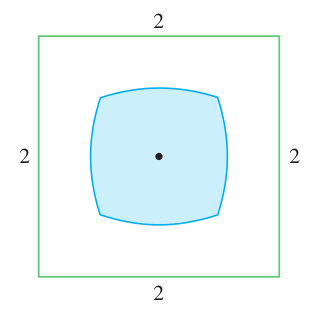
\includegraphics[scale=0.5]{./diagrams/squarish.png}
  \end{figure}
\end{frame}

\begin{frame}
  \frametitle{Substitution to Find Area}
  \begin{description}
  \item[Hint 1] Think of the curve to integrate in terms of the
    diagram on the next slide.
  \item[Hint 2] The definite integral is
    \begin{equation}
      \label{eq:loocooch}
      A=4\int_{0}^{2-\sqrt{2}}\left(x-\sqrt{2}+2\sqrt{1-\sqrt{2}x}\right)\,dx
    \end{equation}
  \end{description}
  The solution is approximately $A=0.87581$.
  % For calculations see Schmierbuch 2573ff and diagram squarish on
  % desmos.
\end{frame}

\begin{frame}
  \frametitle{Substitution to Find Area}
  \begin{figure}[h]
    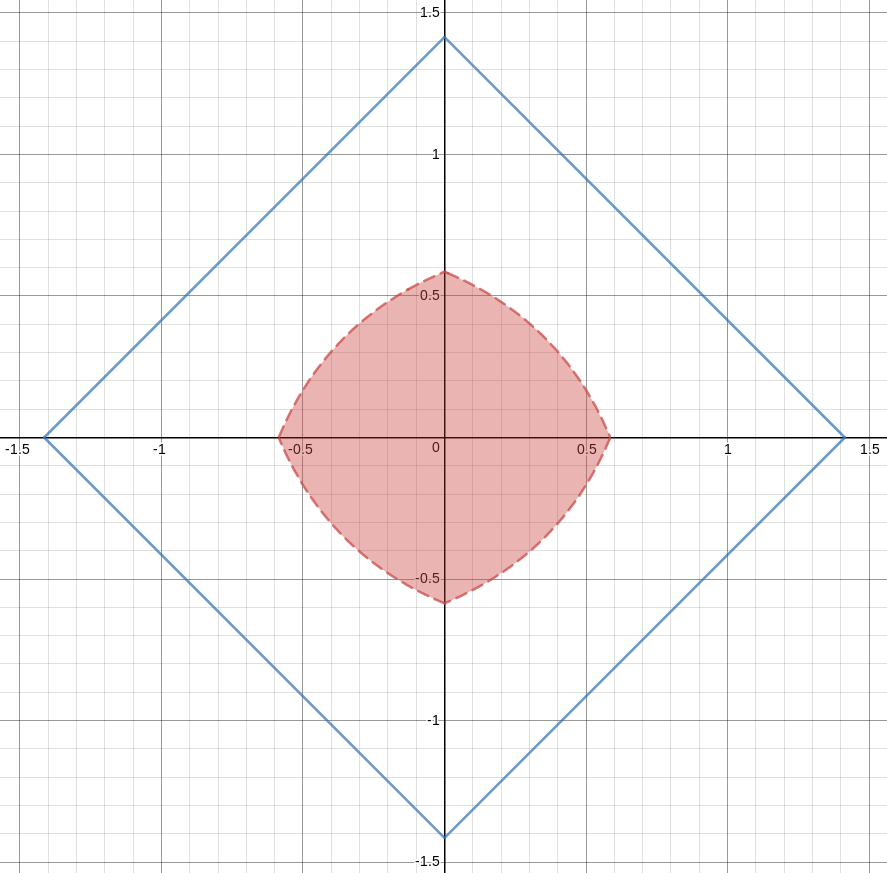
\includegraphics[scale=0.3]{./diagrams/squarish-desmos.png}
  \end{figure}
\end{frame}

% \begin{frame}
%   \frametitle{Finding an Area Solution}
% First, notice that the area $A$ equals
% \begin{equation}
%   \label{eq:aeghieyu}
%   A=(2w)^{2}+8\int_{0}^{w}[g(x)-f(x)]\,dx
% \end{equation}
% where $w$ is the $x$-coordinate of the top right point on the blue
% figure; $f(x)=w$ and $g(x)$ is the function going along the top of the
% blue figure. Since
% \begin{equation}
%   \label{eq:seephoes}
%   1-w=\frac{1}{\sqrt{2}}
% \end{equation}
% it follows that
% \begin{equation}
%   \label{eq:weipeewi}
%   w=1-\frac{1}{\sqrt{2}}
% \end{equation}
% and
% \begin{equation}
%   \label{eq:kehuichu}
%   g(x)=\frac{1-x^{2}}{2}
% \end{equation}
% This appears to be incorrect.
% \end{frame}

\begin{frame}
  \frametitle{Integration Tables}
  Here are integration tables and tables of derivatives to last you
  for a while:
\begin{alltt}
\small
http://www.ambrsoft.com/Equations/Derivation/Derivation.htm
\end{alltt}

\beispiel{Using an Integration Table} Evaluate the indefinite integral
\begin{equation}
  \label{eq:eewuquex}
  \int{}-7\sqrt{\cot{}x}\csc^{2}x\,dx
\end{equation}
The derivative of $f(x)=\cot{}x$ is $f'(x)=-\csc^{2}x$. Using the
substitution $u=\cot{}x$ and $du=-\csc^{2}x\,dx$ yields
\begin{equation}
  \label{eq:qualaiqu}
  \int{}-7\sqrt{\cot{}x}\csc^{2}x\,dx=7\int{}u^{\frac{1}{2}}\,du=\frac{14}{3}\sqrt{\cot^{3}x}+C
\end{equation}
\end{frame}

\begin{frame}
  \frametitle{Integration Table}
  \beispiel{Using an Integration Table} Evaluate the indefinite integral
  \begin{equation}
    \label{eq:xohphohh}
    \int{}\frac{9-9x}{1+x^{2}}\,dx
  \end{equation}
Gather from an integration table (or a table of derivatives) that if
$f(x)=\arctan{}x$ then $f'(x)=1/(1+x^{2})$. Therefore, using the
substitution $u=1+x^{2}$ with $du=2x\,dx$,
\begin{equation}
  \label{eq:mixausho}
  \int{}\frac{9-9x}{1+x^{2}}\,dx=9\cdot\left(\int\frac{1}{1+x^{2}}\,dx-\int\frac{x}{1+x^{2}}\,dx\right)=\notag
\end{equation}
\begin{equation}
  \label{eq:ohleseej}
  9\arctan{}x-\frac{9}{2}\ln\vert{}1+x^{2}\vert{}+C
\end{equation}
\end{frame}

\begin{frame}
  \frametitle{Integration Table}
  \beispiel{Using an Integration Table} Evaluate the indefinite integral
  \begin{equation}
    \label{eq:aigeishu}
    \int\frac{5x}{\sqrt{3-x^{4}}}\,dx
  \end{equation}
Notice in the integration table that
\begin{equation}
  \label{eq:zeecogoo}
  \int\frac{1}{\sqrt{a^{2}-x^{2}}}\,dx=\arcsin\frac{x}{a}+C
\end{equation}
Thus, substituting $u=x^{2}$ and $du=2x\,dx$,
\begin{equation}
  \label{eq:roogheis}
  \int\frac{5x}{\sqrt{3-x^{4}}}\,dx=\frac{5}{2}\arcsin\left(\frac{x^{2}}{\sqrt{3}}\right)+C
\end{equation}
\end{frame}

\begin{frame}
  \frametitle{Exercises for Using an Integration Table}
  {\ubung} Find the following integral.
  \begin{equation}
    \label{eq:ohjomopu}
    \int\frac{1}{\sqrt{8x-x^{2}}}\,dx
  \end{equation}
  Hint: complete the square to find out that $8x-x^{2}=16-(x-4)^{2}$.
\end{frame}

\begin{frame}
  \frametitle{Exercises for Using an Integration Table}
  {\ubung} Find the following integral.
  \begin{equation}
    \label{eq:feecheir}
    \int_{0}^{\frac{\pi}{4}}\frac{1}{1-\sin{}x}\,dx
  \end{equation}
  Hint: expand the fraction by $1+\sin{}x$.
\end{frame}

\begin{frame}
  \frametitle{Exercises for Using an Integration Table}
  {\ubung} Find the following integral.
  \begin{equation}
    \label{eq:dahcohne}
    \int\frac{3x+2}{\sqrt{1-x^{2}}}\,dx
  \end{equation}
\end{frame}

\begin{frame}
  \frametitle{Exercises for Using an Integration Table}
  {\ubung} Find the following integral.
  \begin{equation}
    \label{eq:uokaivie}
    \int_{4}^{(e+1)^{2}}\frac{1}{x-\sqrt{x}}\,dx
  \end{equation}
\end{frame}

\begin{frame}
  \frametitle{Exercises for Using an Integration Table}
For the integral in (\ref{eq:uokaivie}), there are two ways to solve
this problem.
\begin{enumerate}
\item Multiply by the conjugate, simplify, and substitute $u=x-1$.
  Then use formula 29a from Thomas' table of integrals,
  \begin{equation}
    \label{eq:taxeepei}
    \int\frac{1}{x\sqrt{ax+b}}\,dx=\frac{1}{\sqrt{b}}\ln\left\vert\frac{\sqrt{ax+b}-\sqrt{b}}{\sqrt{ax+b}+\sqrt{b}}\right\vert+C
  \end{equation}
\item Substitute $u^{2}=x$. It is generally a good idea to try
  substituting expressions under a square root by $u^{2}$.
\end{enumerate}
The solution for the definite integral is $2$.
\end{frame}

\begin{frame}
  \frametitle{Integration by Parts}
  There is no product rule for integration, so integrals of the form
  \begin{equation}
    \label{eq:auzoowoo}
    \int{}f(x)\cdot{}g(x)\,dx
  \end{equation}
are a problem. Notice, however, that
\begin{equation}
  \label{eq:vieyaigh}
  \left[f(x)g(x)\right]'=f'(x)g(x)+f(x)g'(x)
\end{equation}
and therefore
\begin{equation}
  \label{eq:aiphithe}
  \int{}f'(x)g(x)\,dx+\int{}f(x)g'(x)\,dx=f(x)g(x)+C
\end{equation}
Consequently,
\begin{equation}
  \label{eq:taebohme}
  \int{}f(x)g'(x)\,dx=f(x)g(x)-\int{}f'(x)g(x)\,dx+C
\end{equation}
If we happen to know everything on the right-hand side (RHS), then we
have an integral for the left-hand side (LHS).
\end{frame}

\begin{frame}
  \frametitle{Integration by Parts}
  \beispiel{Integration by Parts} Find
  \begin{equation}
    \label{eq:eecahquo}
    \int{}x\cos{}x\,dx
  \end{equation}
If we choose $f(x)=\cos{}x$ and $g'(x)=x$, then integration by parts
yields
\begin{equation}
  \label{eq:aebashiy}
  \int{}x\cos{}x\,dx=\frac{1}{2}x^{2}\cos{}x+\frac{1}{2}\int{}x^{2}\sin{}x\,dx
\end{equation}
We have not helped our cause. Let's try this the other way around with
$f(x)=x$ and $g(x)=\sin{}x$. Then
\begin{equation}
  \label{eq:oiwuilah}
  \int{}x\cos{}x\,dx=x\sin{}x-\int{}1\cdot\sin{}x\,dx=x\sin{}x+\cos{}x+C
\end{equation}
Success!
\end{frame}

\begin{frame}
  \frametitle{Integration by Parts}
  When we learned integration by substitution, we were able to find
  the antiderivative of $\tan{}x$ and $\cot{}x$. Now it is time to
  find the antiderivative of $\ln{}x$. Use integration by parts for
  \begin{equation}
    \label{eq:xoocheix}
    \int\ln{}x\,dx=\int{}1\cdot\ln{}x\,dx
  \end{equation}
  and find out that
  \begin{equation}
    \label{eq:eimejief}
    \int\ln{}x\,dx=x\ln{}x-x+C
  \end{equation}
Add this integral to your personal list.
\end{frame}

\begin{frame}
  \frametitle{Integration by Parts}
  {\ubung} Evaluate the following integral.
  \begin{equation}
    \label{eq:oizaixea}
    \int{}x^{2}e^{x}\,dx
  \end{equation}
\end{frame}

\begin{frame}
  \frametitle{Integration by Parts}
  {\ubung} Evaluate the following integral.
  \begin{equation}
    \label{eq:nohceira}
    \int{}e^{x}\cos{}x\,dx
  \end{equation}
\end{frame}

\begin{frame}
  \frametitle{Integration by Parts}
  {\ubung} Evaluate the following integral.
  \begin{equation}
    \label{eq:aemahjoo}
    \int\cos^{n}x\,dx
  \end{equation}
  All we want is a \alert{reduction formula} to decrease the exponent
  $n$ to express the integral in terms of $\int\cos^{n-1}x\,dx$.
\end{frame}

\begin{frame}
  \frametitle{Trigonometric Integrals}
  There are several tricks for integrals with trigonometric functions.
  It is best to consult a textbook when you have to solve a particular
  integral. Sometimes we can solve an integral that doesn't involve
  trigonometric functions by substituting trigonometric functions:
  this is called trigonometric substitution. Here is our first
  challenge: solve integrals of the form
  \begin{equation}
    \label{eq:iepheith}
    \int\sin^{m}x\cos^{n}x\,dx
  \end{equation}
\end{frame}

\begin{frame}
  \frametitle{Trigonometric Integrals Case (1)}
  Distinguish two cases: (1) one of the exponents is odd; (2) both
  exponents are even. In case (1), notice that for
  some natural number $k$
  \begin{equation}
    \label{eq:oghufohx}
    \sin^{m}x=\sin^{2k+1}x=(\sin^{2}x)^{k}\sin{}x=(1-\cos^{2}x)^{k}\sin{}x
  \end{equation}
  I have assumed here that the sine has the odd exponent. If the
  sine's exponent is even then use the cosine's exponent instead.
\end{frame}

\begin{frame}
  \frametitle{Trigonometric Integrals Case (1)}
  Let's demonstrate the rest of the procedure by example, using the
  substitution $u=\cos{}x$ and $du=-\sin{}x\,dx$
\begin{equation}
  \label{eq:zephulai}
  \int\sin^{3}x\cos^{2}x\,dx=\int(1-\cos^{2}x)\cos^{2}x\sin{}x\,dx=-\int(1-u^{2})u^{2}\,du=\notag
\end{equation}
\begin{equation}
  \label{eq:joochupa}
  -\int{}u^{2}\,du+\int{}u^{4}\,du=-\frac{1}{3}u^{3}+\frac{1}{5}u^{5}+C=-\frac{1}{3}\cos^{3}x+\frac{1}{5}\cos^{5}x+C\notag
\end{equation}
\end{frame}

\begin{frame}
  \frametitle{Trigonometric Integrals Case (1)}
Here is what happens when the sine's exponent is even. Substitute $u=\sin{}x$ and $du=\cos{}x\,dx$.
\begin{equation}
  \label{eq:siengoel}
  \int\cos^{3}x\sin^{2}x\,dx=\int(1-\sin^{2}x)\sin^{2}x\cos{}x\,dx=\int(1-u^{2})u^{2}\,du=\notag
\end{equation}
\begin{equation}
  \label{eq:daejeile}
  \int{}u^{2}\,du-\int{}u^{4}\,du=\frac{1}{3}u^{3}-\frac{1}{5}u^{5}+C=\frac{1}{3}\sin^{3}x-\frac{1}{5}\sin^{5}x+C\notag
\end{equation}
\end{frame}

\begin{frame}
  \frametitle{Trigonometric Integrals Case (2)}
If both exponents are even, in case (2), remember that
  \begin{equation}
    \label{eq:ielahghu}
    \begin{array}{rcl}
      \cos{}2x & = & \cos^{2}x-\sin^{2}x \\
   \hspace{.5in} & & \\
      1 & = & \cos^{2}x+\sin^{2}x \\
    \end{array}
  \end{equation}
Add and subtract these two equations for
\begin{equation}
  \label{eq:einahkur}
  \begin{array}{rcl}
   \sin^{2}x & = & \frac{1}{2}-\frac{1}{2}\cos{}2x \\
   \hspace{.5in} & & \\
   \cos^{2}x & = & \frac{1}{2}+\frac{1}{2}\cos{}2x \\
  \end{array}
\end{equation}
\end{frame}

\begin{frame}
  \frametitle{Trigonometric Integrals Case (2)}
Substitute (\ref{eq:einahkur}), as in the following example.
\begin{equation}
  \label{eq:owamaela}
  \int\cos^{4}x\sin^{2}x\,dx=\int\left(\frac{1}{2}+\frac{1}{2}\cos{}2x\right)^{2}\cdot\left(\frac{1}{2}-\frac{1}{2}\cos{}2x\right)\,dx\notag
\end{equation}
\begin{equation}
  \label{eq:acahjahj}
  \int\cos^{4}x\sin^{2}x\,dx=\frac{1}{8}\int\left(1+\cos{}2x-\cos^{2}2x-\cos^{3}2x\right)\,dx\notag
\end{equation}
You can use conventional methods and reducing the term involving
$\cos^{2}2x$ again to provide the solution
\begin{equation}
  \label{eq:cohnalee}
  \int\cos^{4}x\sin^{2}x\,dx=\frac{1}{16}\left(x-\frac{1}{4}\sin{}4x+\frac{1}{3}\sin^{3}2x\right)
\end{equation}
\end{frame}

\begin{frame}
  \frametitle{Trigonometric Integrals Case (2)}
You can solve case (2) by using trigonometric identities, as on the
last slide; you can also solve it by using integration by parts. Consider
the example on the next slide.

\bigskip

On the next slide, make sure that the solutions in (\ref{eq:aoyoodof}) and
(\ref{eq:uupheilu}) agree (use the double angle formula for $\sin{}2x$).
\end{frame}

\begin{frame}
  \frametitle{Trigonometric Integrals Case (2)}
Using trigonometric identities,
\begin{equation}
  \label{eq:aoyoodof}
  \int\sin^{2}x\,dx=\int\left(\frac{1}{2}-\frac{1}{2}\cos{}2x\right)\,dx=\frac{1}{2}x-\frac{1}{4}sin{}2x+C
\end{equation}

Using integration by parts,
\begin{equation}
  \label{eq:hezaifoo}
  \int\sin^{2}x\,dx=\int\sin{}x\sin{}x\,dx=-\sin{}x\cos{}x+\int\cos^{2}x\,dx=\notag
\end{equation}
\begin{equation}
  \label{eq:uophaequ}
  -\sin{}x\cos{}x+\int\left(1-\sin^{2}x\right)\,dx=-\sin{}x\cos{}x+x-\int\sin^{2}x\,dx\notag
\end{equation}
Note that for $A=\int\sin^{2}x\,dx$, this means that
\begin{equation}
  \label{eq:uupheilu}
  2A=-\sin{}x\cos{}x+x+C,\mbox{ so }A=-\frac{1}{2}\sin{}x\cos{}x+\frac{1}{2}x+C
\end{equation}
\end{frame}

\begin{frame}
  \frametitle{Exercises}
  {\ubung} Evaluate the following integral.
  \begin{equation}
    \label{eq:uejahgai}
    \int\cos^{3}x\,dx
  \end{equation}
\end{frame}

\begin{frame}
  \frametitle{Exercises}
  {\ubung} Evaluate the following integral.
  \begin{equation}
    \label{eq:ufiurugo}
    \int_{0}^{\frac{\pi}{2}}\sin^{2}x\,dx
  \end{equation}
\end{frame}

\begin{frame}
  \frametitle{Exercises}
  {\ubung} Evaluate the following integral.
  \begin{equation}
    \label{eq:iepahgai}
    \int_{0}^{\frac{\pi}{6}}3\cos^{5}3x\,dx
  \end{equation}
\end{frame}

\begin{frame}
  \frametitle{Exercises}
  {\ubung} Evaluate the following integral.
  \begin{equation}
    \label{eq:koquohge}
    \int_{0}^{\pi}\sqrt{1-\cos{}2x}\,dx
  \end{equation}
  Hint: Use the double-angle formula to get rid of the square root
  sign.
\end{frame}

\begin{frame}
  \frametitle{Exercises}
  {\ubung} Evaluate the following integral.
  \begin{equation}
    \label{eq:thaemooc}
    \int_{-\frac{\pi}{4}}^{\frac{\pi}{4}}16\sin^{2}x\cos^{2}x\,dx
  \end{equation}
\end{frame}

\begin{frame}
  \frametitle{Exercises}
  {\ubung} Evaluate the following integral.
  \begin{equation}
    \label{eq:noojoosh}
    \int_{0}^{\frac{\pi}{2}}35\sin^{4}x\cos^{3}x\,dx
  \end{equation}
\end{frame}

\begin{frame}
  \frametitle{Partial Fractions}
  Find the integral
  \begin{equation}
    \label{eq:xaikieji}
    \int\frac{5x-3}{x^{2}-2x-3}
  \end{equation}
We have no quotient rule for integration, so this integral presents a
challenge. If we could express the rational function as a sum of simpler
fractions, called \alert{partial fractions}, we may be able to solve
this. First, factor the denominator
\begin{equation}
  \label{eq:cichacah}
  x^{2}-2x-3=(x+1)(x-3)
\end{equation}
Then find $A$ and $B$ for
\begin{equation}
  \label{eq:rifiedoh}
\frac{5x-3}{x^{2}-2x-3}=\frac{A}{x+1}+\frac{B}{x-3}
\end{equation}
Getting rid of all the fractions, (\ref{eq:rifiedoh}) is equivalent to
\begin{equation}
  \label{eq:phiethee}
\alert{5}x+\alert{(-3)}=\alert{(A+B)}x+\alert{(B-3A)}
\end{equation}
\end{frame}

\begin{frame}
  \frametitle{Partial Fractions}
  (\ref{eq:phiethee}) is true only when
  \begin{equation}
    \label{eq:oorighoe}
    \begin{array}{rcrcr}
      A&+&B&=&5 \\
      -3A&+&B&=&-3
    \end{array}
  \end{equation}
This system of linear equations has the solution $A=2$ and $B=3$.
Therefore,
\begin{equation}
  \label{eq:vaewahsh}
\int\frac{5x-3}{x^{2}-2x-3}=\int\frac{2}{x+1}\,dx+\int\frac{3}{x-3}\,dx=\notag
\end{equation}
\begin{equation}
  \label{eq:moochofe}
2\ln|x+1|+3\ln|x-3|+C
\end{equation}
\end{frame}

\begin{frame}
  \frametitle{Exercises}
  {\ubung} Use partial fractions to evaluate the following integral.
  \begin{equation}
    \label{eq:feirueho}
    \int\frac{x^{2}+4x+1}{(x-1)(x+1)(x+3)}\,dx
  \end{equation}
\end{frame}

\begin{frame}
  \frametitle{Exercises}
  {\ubung} Use partial fractions to evaluate the following integral.
  \begin{equation}
    \label{eq:ietahpha}
    \int\frac{6x+7}{\left(x+2\right)^{2}}\,dx
  \end{equation}
  Hint: In this case, the denominator for $A$ is $x+2$ and the
  denominator for $B$ is $\left(x+2\right)^{2}$.
\end{frame}

\begin{frame}
  \frametitle{Exercises}
  {\ubung} Use partial fractions to evaluate the following integral.
  \begin{equation}
    \label{eq:saeheing}
    \int\frac{2x^{3}-4x^{2}-x-3}{x^{2}-2x-3}\,dx
  \end{equation}
  Hint: Use polynomial division for
  $2x^{3}-4x^{2}-x-3=2x(x^{2}-2x-3)+(5x-3)$.
\end{frame}

\begin{frame}
  \frametitle{Improper Integrals}
  There are sometimes infinite curves with finite areas under them.
  Consider the following two examples. 
  \begin{figure}[h]
    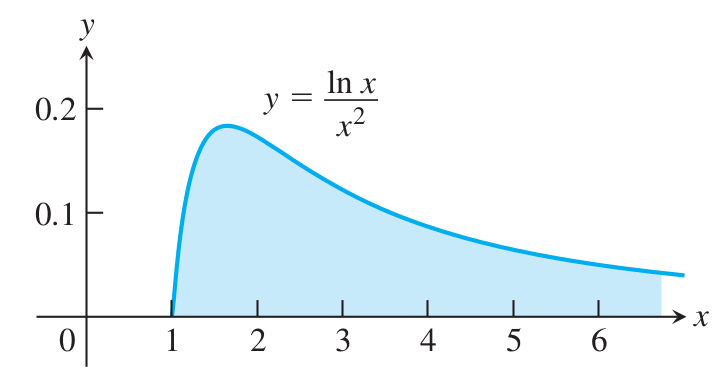
\includegraphics[scale=0.4]{./diagrams/improper1.png}
  \end{figure}
\end{frame}

\begin{frame}
  \frametitle{Improper Integrals}
  There are sometimes infinite curves with finite areas under them.
  Consider the following two examples. 
  \begin{figure}[h]
    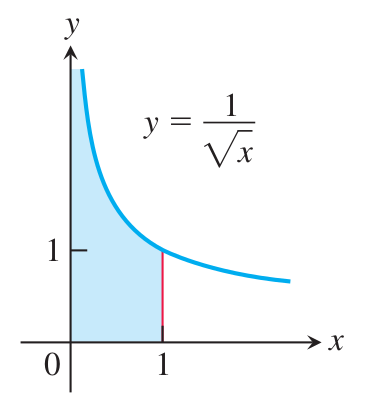
\includegraphics[scale=0.5]{./diagrams/improper2.png}
  \end{figure}
\end{frame}

\begin{frame}
  \frametitle{Improper Integrals}
  \begin{figure}[h]
    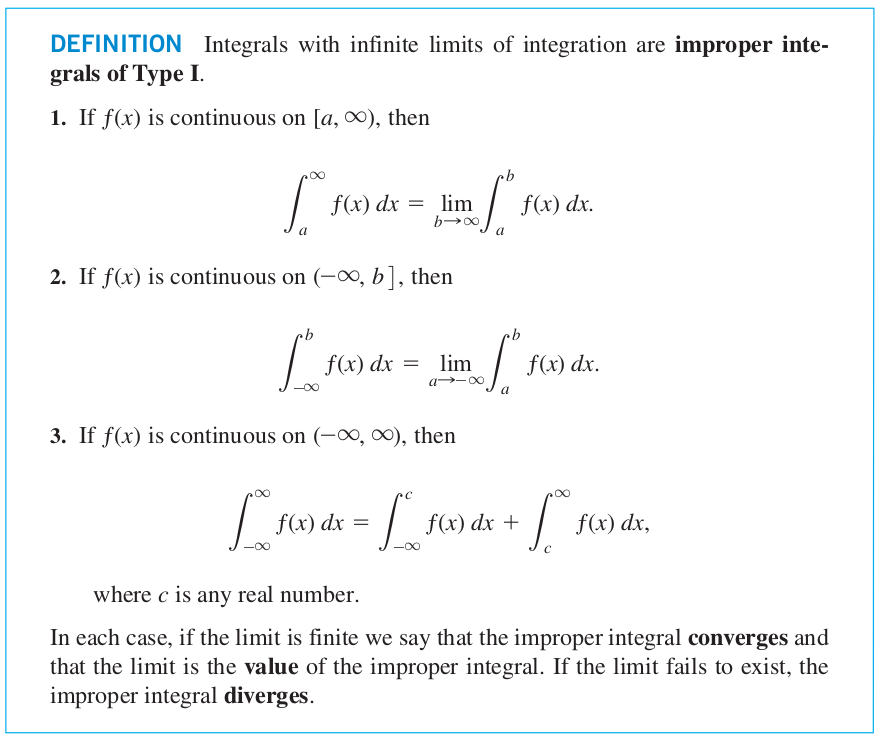
\includegraphics[scale=0.3]{./diagrams/improper3.png}
  \end{figure}
\end{frame}

\begin{frame}
  \frametitle{Improper Integrals}
  \begin{figure}[h]
    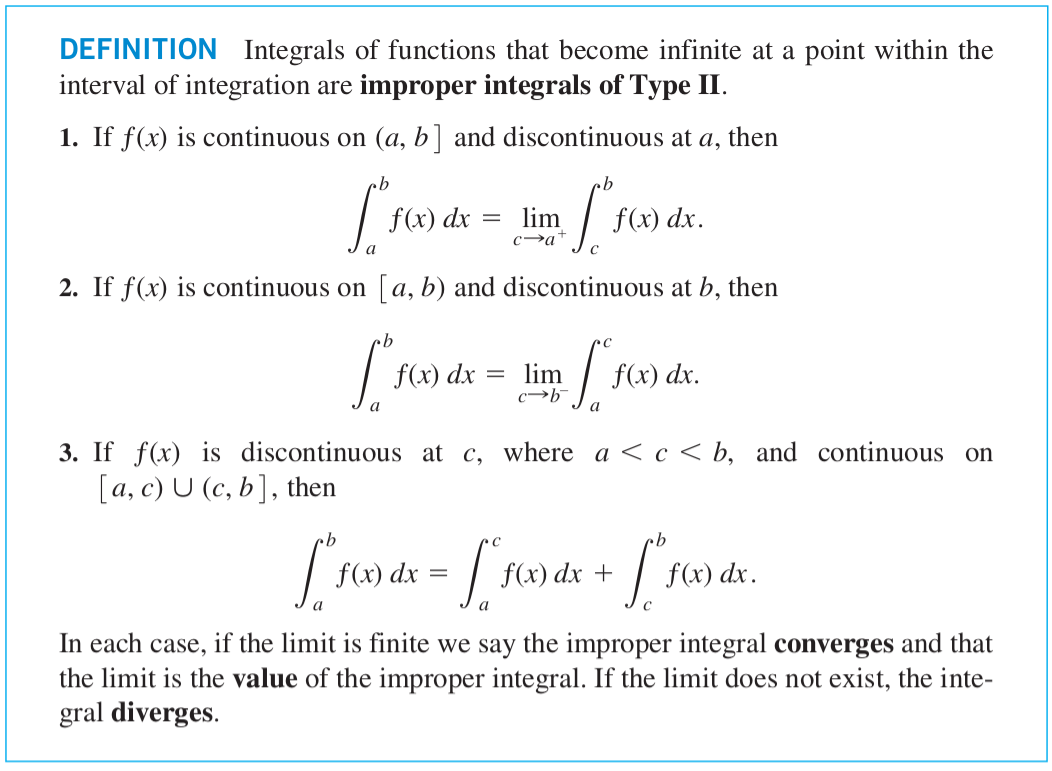
\includegraphics[scale=0.28]{./diagrams/improper4.png}
  \end{figure}
\end{frame}

\begin{frame}
  \frametitle{Improper Integrals Exercises}
{\ubung} Evaluate the improper integral.
  \begin{equation}
    \label{eq:cheifiwo}
    % \int_{0}^{\infty}e^{-\frac{x}{2}}=\lim_{b\rightarrow\infty}\int_{0}^{b}e^{-\frac{x}{2}}
    \int_{0}^{\infty}e^{-\frac{x}{2}}
  \end{equation}
\end{frame}

\begin{frame}
  \frametitle{Improper Integrals Exercises}
{\ubung} Evaluate the improper integral.
  \begin{equation}
    \label{eq:eiquiena}
    \int_{1}^{\infty}\frac{\ln{}x}{x^{2}}\,dx
  \end{equation}
\end{frame}

\begin{frame}
  \frametitle{Improper Integrals Exercises}
{\ubung} Evaluate the improper integral.
  \begin{equation}
    \label{eq:yielohwi}
    \int_{-\infty}^{\infty}\frac{1}{1+x^{2}}\,dx
  \end{equation}
\end{frame}

\begin{frame}
  \frametitle{Improper Integrals Exercises}
{\ubung} Evaluate the improper integral.
  \begin{equation}
    \label{eq:oocoibuo}
    \int_{0}^{1}\frac{1}{1-x}\,dx
  \end{equation}
\end{frame}

\begin{frame}
  \frametitle{Improper Integrals Exercises}
{\ubung} Evaluate the improper integral.
  \begin{equation}
    \label{eq:eebaesie}
    \int_{0}^{3}\frac{1}{(x-1)^{\frac{2}{3}}}\,dx
  \end{equation}
\end{frame}

\begin{frame}
  \frametitle{Improper Integrals Exercises}
{\ubung} Evaluate the improper integral.
  \begin{equation}
    \label{eq:aezihuth}
    \int_{-\infty}^{0}e^{-|x|}\,dx
  \end{equation}
\end{frame}

\begin{frame}
  \frametitle{Improper Integrals Exercises}
{\ubung} Evaluate the improper integral.
  \begin{equation}
    \label{eq:wiexohje}
    \int_{0}^{1}x\ln{}x\,dx
  \end{equation}
\end{frame}

\begin{frame}
  \frametitle{End of Lesson}
Next Lesson: Maclaurin and Taylor Series Expansion
\end{frame}

\end{document}

